\newpage{\clearpage}
\chapter{ Marco te\'{o}rico}

A continuación, se explican los conceptos claves que se deben saber para poder realizar este proyecto. Se inicia explicando las distorsiones en la onda, el factor de potencia y la distorsión armónica total en voltaje y corriente, con el fin de entender como se generan las distorsiones en la onda y como están compuestas. Siguiente a esto, se explica el estándar IEEE 1459 del 2010 que es el objetivo principal del proyecto en donde se explican las condiciones que una carga puede presentar y como se deben analizar estas cargas en dichas condiciones. Se procede a realizar un ejercicio practico en donde se analiza una de las situaciones contempladas en el estándar IEEE 1459 para demostrar la implementación de esta.\\\\
Una vez demostrado el estándar, se procede a crear un software que nos permita realizar los cálculos de este de forma digital y al final mostrar los resultados en una página web. Para lograr este software se requiere tener claro los conceptos de programación orientada a objetos, programación web, definición del Front-end, definición del Back-end y la arquitectura de software REST. De esta manera ya es posible tener todo lo necesario para crear el software.\\\\
Para entender como funcionan la descomposición de onda y el proceso de convertir una señal análoga a digital, es necesario comprender los principios básicos de la transformada de Fourier y el teorema de muestreo de Nyquist-Shannon.\\\\
Por último, se requiere una definición de ¿qué es el internet de las cosas?, ¿qué permite? y ¿qué dispositivos se usan para lograr dicha funcionalidad? Para implementar este concepto, se utilizará la tarjeta raspberry pi, la cual cumple con las características fundamentales para conectar el medidor de energía a la red de internet.

\section{Medidores en la actualidad}

Thomas Alva Edison, al presentó el primer sistema de distribución eléctrico usando corriente alterna, creó un modelo de negocio en dónde la luz se pudiera vender de la misma manera que el gas. Su medidor eléctrico, patentado en Estados Unidos en 1881 usa efectos electroquímicos de corriente cómo método de funcionamiento.\cite{A55}\\\\
Este medidor contenía una celda una celda electrolítica, en donde su ubicaba una lamina de cobre pesada con precisión al inicio del periodo de facturación. A medida que la corriente eléctrica pasaba por la lamina provoca una deposición de cobre. Al finalizar el periodo de facturación se vuelve a pesar el cobre y la diferencia en peso representó la cantidad de electricidad que había pasado. De tal forma se calibró el medidor para que las facturas pudieran expresarse en pies cúbicos de gas.\cite{A55}\\\\
Este medidor se usó hasta el fin del siglo XIX; pese a ello, obtener el valor de la medición era complicado de obtener para la empresa de servicios públicos y aún más para el cliente. Por ende, Edison creó un sistema de conteo para mejorar la lectura de este.\cite{A55}\\\\
En la misma década, otro medidor de energía fue creado usando el principio de oscilación o rotación proporcional a la energía el cual podría conducir a un registro de lectura. Este principio lo crearon los American William Edward Ayrton y John Perry en 1881. En su forma más avanzada, este medidor tenía dos péndulos, con una bobina en ambos péndulos conectados al voltaje. Debajo de los péndulos había dos bobinas de corriente que se enrollaban en direcciones opuestas. Por tanto, uno de los péndulos iba más lento y el otro más rápido que sin carga. La diferencia entre los tiempos de oscilación, promovió el mecanismo de conteo. El rol de los dos péndulos se intercambió cada minuto, de modo que se pudiera compensar la diferencia inicial entre los tiempos de oscilación de los péndulos. Al mismo tiempo, se dio cuerda al reloj.\cite{A55}\\\\
Estos medidores eran costosos porque contenían dos relojes y fueron reemplazados gradualmente por medidores de motor. Los medidores de péndulo miden amperios-hora o vatios-hora, pero solo se pueden usar para corriente continua.\cite{A55}\\\\
Dichos medidores de motor, el par motor es proporcional a la carga y está equilibrado por un par de frenado, de modo que la velocidad del rotor es proporcional a la carga cuando los pares están en equilibrio. El Norte Americano Elihu Thomson, invenó su Wattímetro de grabación en 1889 para General Electric. Era un motor sin hierro, con el rotor estimulado por el voltaje a través de una bobina y una resistencia, usando un conmutador.\cite{A55}\\\\
De tal manera, los medidores fueron mejorando sus características en cuanto su forma de medir la corriente eléctrica y la lectura de esta para los usuarios. Sin embargo, como lo menciona Andrew J Berrisfold en el proyecto del impacto armónico \cite{A43}, dichos medidores no contemplaron la opción que las señales de voltaje y corriente fueran no sinusoidales, lo que conlleva a que las mediciones no puedan ser exactas. \\\\
El estándar IEEE14-59-2010 (1459-2010 IEEE Standard Definitions for the Measurement of Electric Power Quantities Under Sinusoidal, Nonsinusoidal, Balanced, or Unbalanced Conditions., n.d.) explica la forma en cómo se debe obtener las distintas potencias eléctricas en el caso de condiciones desbalanceadas.\\\\
En la tabla (REF:tabla) se enseña algunos de los medidores usados en la actualidad en Colombia y se hace un estudio de su ficha técnica para verificar si estos implementan el estándar IEEE 1459 y si cuentan con una aplicación web para ver las mediciones de este.\\\\

\begin{longtable}{|l|c|c|c|}
    \hline
    Medidor - Fabricante               & \multicolumn{1}{l|}{IEEE 1459} & \multicolumn{1}{l|}{Aplicación web} & \multicolumn{1}{l|}{Referencia} \\ \hline
    \endfirsthead
    %
    \multicolumn{4}{c}%
    {{\bfseries Table \thetable\ continued from previous page}} \\
    \endhead
    %
    MONOFÁSICO BIFILAR -1F2H - RYMEL              & NO & NO & \cite{A56} \\ \hline
    MONOFÁSICO TRIFILAR - 1F3H - RYMEL & \cellcolor[HTML]{FFFFFF}NO     & NO                                  & \cite{A57}                        \\ \hline
    TRIFÁSICO TETRAFILAR - 3F4H-LCD - RYMEL       & NO & NO & \cite{A58} \\ \hline
    BIFÁSICO TRIFILAR - 2F3H-LCD - RYMEL          & NO & NO & \cite{A59} \\ \hline
    Todos los medidores - Iskra                   & NO & NO & \cite{A60} \\ \hline
    Todos los medidores - Skaitek                 & NO & NO & \cite{A61} \\ \hline
    Medidores de energía clase 1 - INELCA         & NO & NO & \cite{A62} \\ \hline
    Aclara I-210+c™ Electricity Meter - Sensus    & NO & SI & \cite{A63} \\ \hline
    Medidores inteligentes tipo SMETS 1 y SMETS 2 & NO & SI & \cite{A64} \\ \hline
    \end{longtable}
Al obtener los resultados de la investigación, los medidores más antiguos no cumplen con los dos criterios propuestos; sin embargo, los medidores inteligentes (Smart Meters), cuentan con aplicaciones web, dónde sus valores pueden ser visualizados, pero estas mediciones no implementan el IEEE1459.\\\\

\section{Factor de potencia y distorsión de la onda.}
% El factor de potencia se puede interpretar como la relación entre la energía transmitida a la carga y la energía máxima que podría transmitirse siempre que las pérdidas de línea se mantengan iguales.\cite{A28}\\  Como un caso base, se considera una carga lineal R-L mostrado en la figura \ref{fig:RL} alimentado por medio de una fuente sinusoidal en estado estable. Usando valores rms para las magnitudes de voltaje y corriente, la potencia suministrada por la fuente es:\cite{A29}\\
Las distorsiones presentes en la onda se interpretan como ruido eléctrico, estas distorsiones es la superposición de señales en múltiplos de la frecuencia fundamental. Muchas de estas distorsiones son generadas por equipos como por ejemplo televisores, computadores, microondas; etc.\\
%  Los armónicos se encuentran en equipos principales generadores de armónicos que efectúan circuitos de rectificación como por ejemplo computadores, televisores, microondas; etc. \cite{A28}\\  Como un caso base, se considera una carga lineal R-L mostrado en la figura \ref{fig:RL} alimentado por medio de una fuente sinusoidal en estado estable. Usando valores rms para las magnitudes de voltaje y corriente, la potencia suministrada por la fuente es:\cite{A29}\\
\begin{equation}\label{EQ1}
P=V_{s}I_{s}cos \phi\\
\end{equation}
El factor de potencia (FP) se puede interpretar como la relación entre la energía transmitida a la carga y la energía máxima que podría transmitirse siempre que las pérdidas de línea se mantengan iguales. \cite{A30} Este se puede expresar como la analogía entre la potencia real media P y el producto de la tensión y corriente rms:\\
% El factor de potencia (FP), se conoce como la analogía entre la potencia real media P y el producto de la tensión y corriente rms:
\begin{equation}\label{EQ2}
PF=\frac{P}{V_{s}I_{s}}=cos\phi\\
$(Usando \ref{EQ1})$  \\
\end{equation} 

Y por lo tanto, la corriente rms es:\\

\begin{equation}\label{EQ3}
I=\frac{P}{V_{s}PF}\\
$(Usando \ref{EQ2})$  \\
\end{equation} 

Esto demuestra que el PF y la corriente $I_{s}$ son inversamente proporcional. \\

\begin{figure}[H]
\centering
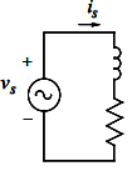
\includegraphics{2Marco/CargaRL}
\caption{ Circuito RL  } \cite{A29} 
\label{fig:RL}
\end{figure} 


%\begin{equation}\label{eq1}
%E_{c}=\frac{1}{2}m v^2\\
%\end{equation}
%Donde:\\\\
%$E_{c}$: Energía Cinética\\
%$m$: Masa Propia Del Aire\\
%$v$: Velocidad Propia Del Aire.\\


\section{Distorsión armónica total (THD) y valor RMS de la corriente distorsionada}


Una señal de corriente sinusoidal para una carga lineal como se muestra en la figura \ref{fig:RL}, no tiene distorsión, sin embargo, hay señales de corrientes que su forma de onda es distorsionada debido a el proceso de rectificar la corriente alterna en corriente directa, haciendola no sinusoidal, es decir la onda se distorsiona. \cite{A29} Un ejemplo de una señal con distorsión se puede ver en la figura \ref{fig:distorsion_current} en donde $i_{s}$ es la señal de corriente distorsionada y $V_{s}(t)$ es sinusoidal. El análisis se aplica a la utilidad de suministros ya sean en monofásico o trifásico, en donde el estudio se realiza por fases.\\
  
\begin{figure}[H]
\centering
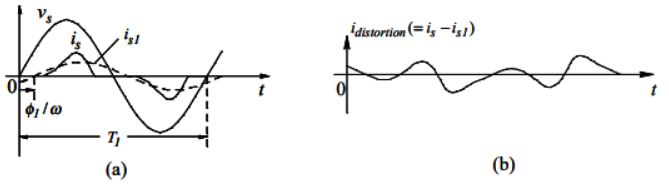
\includegraphics{2Marco/distorsin}
\caption{ Señal de corriente con distorsión: (a) Fase de la corriente y su componente fundamental; (b) Componente de distorsión} \cite{A29} 
\label{fig:distorsion_current}
\end{figure} 



La onda periódica de la corriente $i_{s}(t)$, se puede expresar en componentes de Fourier:\\
\begin{equation}\label{EQ4}
i_{s}(t)=i_{s1}(t) + \sum_{h=2}^{\infty}i_{sh(t)}\\
\end{equation}
Donde:\\
$\sum_{h=2}^{\infty}i_{sh(t)} = i_{distorsion}(t)$\\

El componente dc se asume como cero e $i_{s}$ es la componente fundamental mostrada en la figura \ref{fig:distorsion_current}(a). Partiendo de la ecuación \ref{EQ4} la componente de distorsión en la corriente es la diferencia entre $i_{s}(t)$ y su componente de frecuencia fundamental:\cite{A29}\\  
 
\begin{equation}\label{EQ5}
i_{distorsión}(t)=i_{s}(t)-i_{s1}(t)\\
\end{equation}

En una forma de onda con su frecuencia de línea $f_{1}$ y su tiempo de periodo $T_{1}(=\frac{1}{f_{1}})$, los componentes en la expresión de \ref{EQ5} son en los múltiplos de $h$ en la frecuencia fundamental, como por ejemplo, el $3^{er}$ armónico $(h=3)$ está en $180 Hz$ con un sistema de $60 Hz$.\cite{A29}\\

Un concepto básico que se usa es que en una forma de onda repetitiva, la integral de el producto de dos componentes armónicos (incluyendo la fundamental) en frecuencias desiguales sobre repeticiones del tiempo de periodo es igual a cero: \cite{A29}\\

\begin{equation}\label{EQ6}
\int_{T_{1}}^{}f_{h1}(t) \cdot g_{h2}(t) \cdot dt = 0\\
\end{equation}
Donde:\\
$h1 \neq h2$\\

Con el fin de obtener el valor rms de $i_{s}(t)$ en la figura \ref{fig:distorsion_current}(a), se aplica el concepto básico de rms:\\

\begin{equation}\label{EQ7}
I_{s}=\sqrt{\frac{1}{T_{1}}\int_{T_{1}}^{}(i_{s})^2(t) \cdot dt}\\
\end{equation}


Donde, de la ecuación \ref{EQ4}\\

\begin{equation}\label{EQ8}
i^2_{s}=(i_{s1}+ (\sum_{h=2}^{\infty}i_{sh})^2 = i^2_{sh} + \sum_{h=2}^{\infty}i^2_{sh(t)} \\ 
$+ productos en términos de frecuencia de cruce$
\end{equation}

Sustituyendo la ecuación \ref{EQ8} en la ecuación \ref{EQ7}, con el concepto visto en la ecuación \ref{EQ6}, cada integral de las frecuencias cruzadas es igual a cero,

\begin{equation}\label{EQ9}
I_{s} = \sqrt{\frac{1}{T}\int_{T_{1}}^{}i^2_{s1}(t) \cdot dt + \sum_{h=2}^{\infty}\frac{1}{T_{1}}\int_{T1}^{}i^2_{sh}(t)\cdot dt}\\
\end{equation}
Donde:\\
$\frac{1}{T}\int_{T_{1}}^{}i^2_{s1}(t) \cdot dt = I^2_{sh1}$\\\\
$\sum_{h=2}^{\infty}\frac{1}{T_{1}}\int_{T1}^{}i^2_{sh}(t)\cdot dt = I^2_{distorsion}$\\\\
Por lo tanto,\\
\begin{equation}\label{EQ10}
I_{s} = \sqrt{I^2_{s1}+I^2_{distorsion}}\\\\
\end{equation}

Donde los valores rms del componente de la frecuencia fundamental y los componentes de distorsión son los siguientes:\\
\begin{equation}\label{EQ11}
I_{s1}=\sqrt{\frac{1}{T}\int_{T1}^{}i^2_{s1}(t) \cdot dt}\\
\end{equation}
y\\
\begin{equation}\label{EQ12}
I_{distorsion}=\sqrt{\sum_{h=2}^{\infty}\left(\frac{1}{T_{1}}\int_{T_{1}}^{}i^2_{sh}(t)\cdot dt\right)}=\sqrt{\sum_{h=2}^{}I^2_{sh}}\\\\
\end{equation}

La ecuación descrita anteriormente, presenta que el valor rms de la componente de distorsión en la figura \ref{fig:distorsion_current} puede ser obtenido de s valores de las componentes individual de los armónicos.\cite{A29}\\

Tomando como referencia los valores rms de los componentes de la distorsión y la fundamental en la corriente $i_{s}(t)$, un indice de distorsión llamado Distorsión Armónica Total (THD) es definida en porcentaje y este mismo pude ser presentado en distintas formas bajo las siguientes ecuaciones:\\

\begin{equation}\label{EQ13}
\%THD = 100*\frac{I_{distorsion}}{I_{s1}}\\
=100*\frac{\sqrt{I^2_{s}-I^2_{s1}}}{I_{s1}}\\
=100*\frac{\sqrt{\sum_{h=2}^{\infty}I^2_{sh}}}{I_{s1}}\\
\end{equation}



\section{ Definiciones del STD IEEE 1459 para la medición de calidad energética bajo condiciones balanceadas y des balanceadas }
\subsection{Mono-fase}
\subsubsection{Mono-fase sinusoidal}

Se parte de una entrada de tipo sinusoidal:\\
\begin{equation}\label{EQ14}
v=\sqrt{2}V sin(\omega t)\\
\end{equation}

Y si a esta, se le conecta una carga lineal, se producirá una corriente sinusoidal de tipo:\\

\begin{equation}\label{EQ15}
i\sqrt{2}I sin(\omega t - \theta)\\
\end{equation}

Donde:\\
$V$ es el valor rms de el voltaje $(V)$\\
$I$ es el valor rms de el voltaje $(I)$\\
$\omega$ es la frecuencia angular  $2\pi f(rad/s)$\\
$f$ es la frecuencia del sistema $(Hz)$\\
$\theta$ es el ángulo de fase entre el voltaje y la corriente  $(rad)$\\
$t$ es el tiempo $(s)$\\
\subsubsection{Potencia activa(W)}

La potencia activa P o también conocida como potencia real, es la medición del flujo de energía durante un intervalo de tiempo $\tau$ a $\tau + KT$. \cite{A30}\\

\begin{equation}\label{EQ16}
P=\frac{1}{KT}\int_{\tau}^{\tau + KT}pdt = \frac{1}{KT}\int_{\tau}^{\tau + KT}p_{a}dt\\
\end{equation}

Donde:\\
$T=1/f$ es el ciclo de tiempo $(s)$\\
$k$     es un número entero positivo $(s)$\\
$\tau$  es el momento cuando empieza la medición $(s)$\\
$P=VIcos \theta$\\
\subsubsection{Potencia Reactiva (var)}

La magnitud de la potencia reactiva $Q$ iguala la amplitud de la potencia reactiva instantánea $P_{q}$.\cite{A30}\\
\begin{equation}\label{EQ17}
Q=VIsin \theta\\
\end{equation}
\begin{equation}\label{EQ18}
Q=\frac{\omega}{KT}\int_{\tau}^{\tau + KT}i\left[\int_{}^{}vdt\right] dt\\
\end{equation}

Sí la carga es inductiva, entonces $Q>0$. Sí la carga es capacitiva, entonces $Q<0$. Por lo tanto, cuando la corriente atrasa el voltaje $\theta>0$ y viceversa.\\
\subsubsection{Potencia Aparente (VA)}

La potencia aparente $S$ es el producto del voltaje rms y corriente rms.\cite{A30}\\

\begin{equation}\label{EQ19}
S=VI
\end{equation}

$S=\sqrt{P^2+Q^2}$ \\

La potencia aparente de una carga monofásica se puede interpretar como la potencia activa total que se puede transmitir a través de la misma línea mientras se mantiene el voltaje rms constante de la carga y a línea de alimentación  de pérdida de potencia constante.\cite{A30}\\

\subsubsection{Factor de potencia}

\begin{equation}\label{EQ20}
PF=\frac{P}{S}
\end{equation}

El factor de potencia se puede interpretar como el radio entre la energía transmitida a la carga sobre la energía máxima que podría transmitirse, siempre y cuando las pérdidas de línea se mantengan iguales.\cite{A30}\\

Para un $S$ y $V$ dados, la utilización máxima de la línea es obtenida cuando $P=S$, por lo tanto, el radio $P/S$ es un indicador de factor de utilización.\cite{A30}\\
 \subsubsection{Potencia Compleja (VA)}
 
 La potencia compleja es una cantidad la cual la potencia activa es la parte real y la potencia reactica es la parte imaginaría.\cite{A30}\\
 
 \begin{equation}\label{EQ21}
 S = P+jQ =  VI^*\\
\end{equation}  

Esta expresión proviene del triángulo de potencias $S,P$ Y $Q$. En la figura \ref{fig:triangulo} se observa un resumen de las direcciónes del flujo de potencia. El ángulo $\theta$ es el ángulo de fase de la impedancia equivalente compleja $Z/ \theta = \textbf{V/I}$.\cite{A30}\\ 

\begin{figure}[H]
\centering
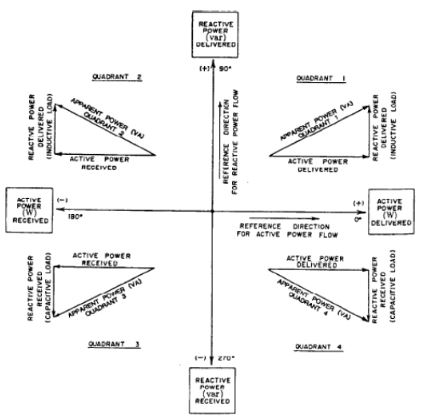
\includegraphics[width = 18cm]{2Marco/triangulopotencias}
\caption{ Cuatro cuadrantes de las direcciónes del flujo de potencia} \cite{A30} 
\label{fig:triangulo}
\end{figure} 


\subsection{Mono-fase no sinusoidal}

Para condiciones estables, una señal de corriente o voltaje no sinusoidal periódica, tiene dos componentes distintos: Los componentes del sistema de frecuencia $V_{1}$ e $i_{1}$ y el término restante $v_{H}$ e $i_{H}$.\cite{A30}\\

\begin{equation}\label{EQ22}
v=v_{1}+v_{H} 
\end{equation}
e\\\\
$i=i_{1}+i_{H}$\\\\
Donde:\\\\
$v_{1}=\sqrt{2V_{1}}sin(\omega t - \alpha_{1})$\\\\
$i_{1}=\sqrt{2I_{1}}sin(\omega t - \beta_{1})$\\\\
$v_{H}=V_{0}+\sqrt{2}\sum_{h\neq 1}^{}V_{h}sin(h\omega t-\alpha_{h})$\\\\
$i_{H}=I_{0}+\sqrt{2}\sum_{h\neq 1}^{}I_{h}sin(h\omega t-\beta_{h})$\\\\

Los valores valores rms al cuadrado son los siguientes:

\begin{equation}\label{EQ59}
\begin{split}
V^2 = {V_{1}}^2 + {V_{H}}^2 \\
I^2 = {I_{1}}^2 + {I_{H}}^2
\end{split}
\end{equation}

Las formas de ondas distorsionadas de a menudo contienen componentes de frecuencias llamadas armónicos. Un grupo especial de inter-armónicos es caracterizado por $h<1$. Estos armónicos tienen periodos más largos que el periodo $T$ de la frecuencia fundamental.\cite{A30}\\

Si la onda distorsionada de corriente y voltaje está compuesta únicamente de armónicos, la medición en intervalos de tiempo $kT$, permitirá una medición correcta de rms y valores de potencia. \cite{A30}\\

Si al menos uno de los inter-armónicos de orden $h$ es irracional, la onda observada no es periódica. En tal caso las mediciones deberían ser infinitas con el fin de tener una medición correcta del rms y las potencias.\cite{A30}\\

\subsubsection{Distorsión Total Armónica (THD) } 

La desviación en general de una onda distorsionada, se puede estimar con la ayuda de la distorsión armónica total. La distorsión armónica total del voltaje es el siguiente:\\

\begin{equation}\label{EQ23}
THD_{v}=\frac{V_{H}}{V_{1}}=\sqrt{\left(\frac{V}{V_{1}}\right)^2-1}\\
\end{equation}

La distorsión armónica total de corriente es el siguiente:\\
\begin{equation}\label{EQ24}
THD_{I}=\frac{I_{H}}{I_{1}}=\sqrt{\left(\frac{I}{I_{1}}\right)^2-1}\\
\end{equation}

\subsubsection{Potencia Activa (W)}

\begin{equation}\label{EQ25}
P=\frac{1}{kT}\int_{\tau}^{\tau + kT}pdt=\int_{\tau}^{\tau + kT}p_{a}dt\\
\end{equation}
$P=P_{1}+P_{H}$\\

\subsubsection{Potencia activa fundamental (W)}


\begin{equation}\label{EQ26}
P_{1}=\frac{1}{kT}\int_{\tau}^{\tau + kT}v_{1}i_{1}dt=V_{i}I_{1}cos \theta_{1}
\end{equation}

\subsubsection{Potencia Aparente (VA)}

\begin{equation}\label{EQ27}
S=VI\\
\end{equation}

La potencia aparente es la cantidad de potencia activa que pueden ser suministradas a la carga en condiciones ideales.\cite{A30}\\

\subsubsection{Potencia aparente fundamental (VA)}

La potencia fundamental $S_{1}$ y sus componentes $P_{1}$ y $Q_{1}$ son las cantidades actuales que ayudan a definir el tipo de flujo del campo magnético asociado con el voltaje y la corriente fundamental.\cite{A30}\\

\begin{equation}\label{EQ28}
S_{1}=V_{1}I{1}
\end{equation}

\subsubsection{Potencia Aparente no fundamental}

\begin{equation}\label{EQ29}
S_{N}=\sqrt{S^2-S^2_{1}}
\end{equation}

También se puede expresar mediante la siguiente ecuación:

\begin{equation}\label{EQ30}
S^2_{N}=D^2_{I}+D^2_{V}+S^2_{H}\\
\end{equation}

\subsubsection{Potencia de la Distorsión de Corriente (var)}
\begin{equation} \label{EQ60}
D_{1}=V_{1}I_{H}=S_{1}(THD_{I})
\end{equation}

\subsubsection{Potencia de la Distorsión de Volatje (var)}
\begin{equation} \label{EQ61}
D_{v}=V_{H}I_{1}=S_{1}(THD_{V})
\end{equation}

\subsubsection{Potencia de la Armónica Aparente (VA)}
\begin{equation} \label{EQ62}
S_{H}=V_{H}I_{H}=S_{1}(THD_{I})(THD_{V})
\end{equation}


\subsubsection{Potencia de distorsión armónica (var)}

\begin{equation}\label{EQ31}
D_{H}=\sqrt{S^2_{H}-P^2{H}}\\
\end{equation}

\subsubsection{Potencia no activa (var)}

\begin{equation}\label{EQ32}
N=\sqrt{S^2-P^2}\\
\end{equation}

Esta potencia agrupa componentes no activas fundamentales y no fundamentales.\cite{A30}\\

\subsubsection{Factor de potencia fundamental}

\begin{equation}
P_{F1}=cos \theta_{1} = \frac{P_{1}}{S_{1}}\\
\end{equation}

Este radio, facilita la evaluación de las condiciones del flujo energía.\cite{A30}\\

\subsubsection{Factor de potencia}

\begin{equation}\label{EQ33}
PF=\frac{P}{S}
\end{equation}

Dados un $S$ y un $V$, la máxima utilización de la línea es obtenido cuando $P=S$, por lo tanto, el radio $P/S$ es un indicador de factor de utilización.\cite{A30}\\

Cuando el $THD_{v}<5\%$ y $THD_{i}>40\%$, es conveniente usar la siguiente ecuación:\\

\begin{equation}\label{EQ34}
PF=\frac{1}{\sqrt{1+THD^2_{I}}}PF_{1}\\
\end{equation}

\subsection{Ejemplo monofásico}

En un circuito de alimentación monofásico se tienen las siguientes medidas tomadas por un analizador de redes eléctricas: $V_{Total}=120 V$;  $THD_{i}= 45\%$; $THD_{v}= 4\%$; $S_{1}= 200 + j40 VA$.\\

Estimar de acuerdo a los criterios de la norma IEEE 1459 las magnitudes de los siguientes parámetros: $V_{1}$, $I_{1}$, $P_{1}$, $Q_{1}$, $S_{T}$, $P_{T}$, $V_{h}$, $I_{h}$, $D_{V}$, $D_{i}$, $S_{h}$.\\

Según la ecuación \ref{EQ19}:\\

$S_{1} = \sqrt{P^2 + Q^2}; \;\;\;\;\;\; S_{1} = \sqrt{200^2 + 40^2} $\\

\textbf{* }$S_{1} = 203,9608 VA$\\

Según la ecuación \ref{EQ23}:\\

$THD_{v}=\sqrt{\left(\frac{V}{V_{1}}\right)^2-1} ;  \;\;\;\;\;\; {THD_{v}}^2=\left(\frac{V}{V_{1}}\right)^2 - 1;  \;\;\;\;\;\;
{THD_{v}}^2=\frac{{V}^2 - {{V}_{1}}^2}{{V_{1}}^2} $\\

${THD_{v}}^2*{{V_{1}}^2}={{V}^2 - {{V}_{1}}^2}; \;\;\;\;\;\;
{THD_{v}}^2*{{V_{1}}^2} + {{V}_{1}}^2={{V}^2}; \;\;\;\;\;\;
{V_{1}}^2 ({THD_{v}}^2 + 1)={{V}^2}; \;\;\;\;\;\;$\\

${V_{1}}^2 = \frac{{{V}^2}}{{THD_{v}}^2 + 1}; \;\;\;\;\;\;
V_{1} = \sqrt{\frac{{{V}^2}}{{THD_{v}}^2 + 1}}; \;\;\;\;\;\;
V_{1} = \sqrt{\frac{{{120V}^2}}{{0.04}^2 + 1}}$\\

\textbf{* }$V_{1} = 119.9041V$\\

$V_{H} = THD_{v}*V_{1};  \;\;\;\;\;\;
V_{H} = 0.04 * 119.9041V$\\

\textbf{* }$V_{H} = 4,7962 V$\\

Según la ecuación \ref{EQ28}:\\

$S_{1} = V_{1}*I_{1}; \;\;\;\;\;\;
I_{1} = \frac{S_{1}}{V_{1}}; \;\;\;\;\;\;
I_{1} = \frac{203,9608VA}{119,9041V}$\\

\textbf{* }$I_{1} = 1,7010A$\\

$I_{H} = THD_{I} * I_{1}; \;\;\;\;\;\;
I_{H} = 0,45 * 1,7010A$\\

\textbf{* }$I_{H} = 0,7654A$\\

Según la ecuación \ref{EQ59}:\\

$I^2 = {I_{1}}^2 + {I_{H}}^2; \;\;\;\;\;\;
I = \sqrt{{I_{1}}^2 + {I_{H}}^2}; \;\;\;\;\;\;
I = \sqrt{{1,7010A}^2 + {0,7654A}^2}$\\

\textbf{* }$I = 1,8653A$\\

Según la ecuación \ref{EQ28}: \\

$S = V*I; \;\;\;\;\;\;
S = 119,9041V * 1,8653A$\\

\textbf{* }$S = 223,836VA$\\

$S_{H} = V_{H}*I_{H}; \;\;\;\;\;\;
\textbf{* }S_{H} = 4,7962V * 0,7654A = 3,6710VA$\\

Según la ecuación \ref{EQ29}: \\

$S_{N} = \sqrt{{S}^2 - {{S}_{1}}^2}; \;\;\;\;\;\;
S_{N} =  \sqrt{{223,836VA}^2 - {203,9608VA}^2}$\\

\textbf{* }$S_{N} = 92,2094VA$\\

Según la ecuación \ref{EQ60}: \\

\textbf{* }$D_{i} = V_{1}*I_{H} = 119,9041V * 0,7654A = 91,7745VA$\\

\textbf{* }$D_{v} = V_{H}*I_{1} = 4.7962V *1,7010A = 8,1583VA$\\

Según la ecuación \ref{EQ26}: \\

$P_{1} = V_{1}*I_{1}*cos \theta_{1}; \;\;\;\;\;\; 
\theta_{1} =  cos^{-1}(\frac{P_{1}}{V_{1}*I_{1}}); \;\;\;\;\;\; 
\theta_{1} =  cos^{-1}(\frac{200VA}{119,9041V*1,7010A})$\\

\textbf{* }$\theta_{1} = 11,3044º$\\

Según la ecuación \ref{EQ33}: \\

$PF_{1} = \frac{P_{1}}{S_{1}}; \;\;\;\;\;\; PF_{1} = \frac{203,9608VA}{200VA};$\\

\textbf{* }$PF_{1} = 0,9805$

Según la ecuación \ref{EQ34}: \\

$PF=\frac{1}{\sqrt{1+THD^2_{I}}}PF_{1}; \;\;\;\;\;\; PF=\frac{1}{\sqrt{1+0,45^2}}0,9805$ \\

\textbf{* } $PF= 0,8941$

Según la ecuación \ref{EQ33}: \\

$PF= \frac{P}{S}; \;\;\;\;\;\; P = PF * S; \;\;\;\;\;\; P = 0,8941 * 223,836 VA$\\

\textbf{* } $P = 200,1317VA$ \\

Según la ecuación \ref{EQ32}: \\

$N=\sqrt{S^2-P^2}; \;\;\;\;\;\; \sqrt{223,836VA^2-200,1317VA^2}$\\

\textbf{* }$N = 100,2489 VAR$\\

Según la ecuación \ref{EQ25}: \\

$P_{H} = P - P_{1}; \;\;\;\;\;\;\; P_{H} = 200,1317VA - 200VA$\\

\textbf{* }$P_{H} = 0,1317VA$

Según la ecuación \ref{EQ31}: \\

$D_{H}=\sqrt{S^2_{H}-P^2{H}}; \;\;\;\;\;\;\; D_{H} = \sqrt{3,6710VA^2 - 0,1317VA^2}$\\

\textbf{* }$D_{H} = 3,6686VAR$\\

En la tabla \ref{tab:resultados-monofasico}, se relacionan los resultados obtenidos del ejemplo anterior.

\begin{table}[H]
\begin{tabular}{|l|l|l|l|l}
\cline{1-4}
Parametro & Total (T)      & Fundamental (1)            & No fundamental (H)               &  \\ \cline{1-4}
V (V)     & 120            & 119,9041                   & 4,7962                           &  \\ \cline{1-4}
I (A)     & 1,8653         & 1,701                      & 0,7654                           &  \\ \cline{1-4}
$THD_{V}$ (\%) & 4              & \multicolumn{1}{c|}{\cellcolor[HTML]{C0C0C0}} & \multicolumn{1}{c|}{\cellcolor[HTML]{C0C0C0}} &  \\ \cline{1-4}
$THD_{I}$ (\%) & 45             & \multicolumn{1}{c|}{\cellcolor[HTML]{C0C0C0}} & \multicolumn{1}{c|}{\cellcolor[HTML]{C0C0C0}} &  \\ \cline{1-4}
P (W)     & 200,1317       & 200                        & 0,1317                           &  \\ \cline{1-4}
Q (VAR)   & \multicolumn{1}{c|}{\cellcolor[HTML]{C0C0C0}} & 40                         & \multicolumn{1}{c|}{\cellcolor[HTML]{C0C0C0}} &  \\ \cline{1-4}
S (VA)    & 223,836        & 203,9608                   & 3,671                            &  \\ \cline{1-4}
$S_{N}$ (VA)   & 92,2094        & \multicolumn{1}{c|}{\cellcolor[HTML]{C0C0C0}} & \multicolumn{1}{c|}{\cellcolor[HTML]{C0C0C0}} &  \\ \cline{1-4}
$D_{I}$ (VA)   & 91,7745        & \multicolumn{1}{c|}{\cellcolor[HTML]{C0C0C0}} & \multicolumn{1}{c|}{\cellcolor[HTML]{C0C0C0}} &  \\ \cline{1-4}
$D_{V}$ (VA)   & 8,1583         & \multicolumn{1}{c|}{\cellcolor[HTML]{C0C0C0}} & \multicolumn{1}{c|}{\cellcolor[HTML]{C0C0C0}} &  \\ \cline{1-4}
$\theta$ (°)  & \multicolumn{1}{c|}{\cellcolor[HTML]{C0C0C0}} & 11,3044                    & \multicolumn{1}{c|}{\cellcolor[HTML]{C0C0C0}} &  \\ \cline{1-4}
PF        & 0,8941         & 0,9805                     & \multicolumn{1}{c|}{\cellcolor[HTML]{C0C0C0}} &  \\ \cline{1-4}
N (VAR)   & 100,2489       & \multicolumn{1}{c|}{\cellcolor[HTML]{C0C0C0}} & \multicolumn{1}{c|}{\cellcolor[HTML]{C0C0C0}} &  \\ \cline{1-4}
$D_{H}$ (VAR)  & 3,6686         & \multicolumn{1}{c|}{\cellcolor[HTML]{C0C0C0}} & \multicolumn{1}{c|}{\cellcolor[HTML]{C0C0C0}} &  \\ \cline{1-4}
\end{tabular}
\caption{Resultado del ejemplo monofásico no sinusoidal}
\label{tab:resultados-monofasico}
\end{table}

\subsection{Sistema trifásico sinusoidal balanceado }

Para este caso se asume un sistema de secuencia positiva rotativa en sentido anti-horario, a, b, c, lo voltaje linea a neutro son los siguientes:

\begin{equation}\label{EQ35}
v_{a}=\sqrt{2}V sin(\omega t)\\
\end{equation} 
$v_{b}=\sqrt{2}V sin(\omega t-120^{\circ})$\\
$v_{c}=\sqrt{2}V sin(\omega t+120^{\circ})$\\

Las líneas de corriente tienen ecuaciones similares, las cuales son:

\begin{equation}\label{EQ36}
i_{a}=\sqrt{2}I sin(\omega t-\theta)\\
\end{equation} 
$i_{b}=\sqrt{2}I sin(\omega t-\theta -120^{\circ})$\\
$i_{c}=\sqrt{2}I sin(\omega t-\theta +120^{\circ})$\\

En sistemas trifásicos balanceados y perfectamente sinusoidal, los sistemas de bajo voltaje no son comunes, solo bajo condiciones de laboratorio en donde se usan amplificadores de potencia de baja distorsión.\cite{A30}\\

En el caso de un sistemas de tres líneas, con voltajes línea a neutro son definidas asumiendo un nodo neutral artificial, el cual se obtienen con ayuda de tres resistencias idénticas conectadas en \textbf{Y}.

\subsubsection{Potencia activa (w)} 
\begin{equation}\label{Eq37}
P=\frac{1}{kT}\int_{\tau}^{\tau +kT}pdt\\
\end{equation}
$P=3VI\cos\theta=\sqrt{3}V_{\ell \ell}I\cos\theta$\\
Donde\\
$V$              es el voltaje rms de línea a neutro\\
$V_{\ell \ell}$  es el voltaje rms línea a línea\\

\subsubsection{Potencia reactiva}


\begin{equation}\label{EQ38}
Q=3VI\sin\theta=\sqrt{3}V_{\ell \ell}I\sin\theta\\
\end{equation}
$|Q|=\sqrt{S^2-P^2}$\\

\subsubsection{Potencia aparente}

\begin{equation}\label{EQ39}
S=3VI=\sqrt{3}V_{\ell \ell}I\\
\end{equation}

\subsubsection{Factor de potencia}

\begin{equation}\label{EQ40}
PF=\frac{P}{s}\\
\end{equation}

\subsection{Sistema trifásico sinusoidal no balanceada}

En este caso, los tres hilos de corriente \textbf{$I_{a},I_{b}$} y \textbf{$I_{c}$}, no tienen las mismas magnitudes y no están desplazadas exactamente $120^{\circ}$ con respecto una a la otra. Las cargas no balanceadas  conlleva a corrientes asimétricas que a su vez causan asimetría de voltaje. En algunas ocasiones sucede que los tres fasores de voltaje no son simétricos. Esto conduce a corrientes asimétras incluso cuando la carga está perfectamente balanceada.\cite{A30}\\


Las ecuaciones de voltaje línea a neutro son los siguientes:

\begin{equation}\label{EQ41}
v_{a}=\sqrt{2}V_{a}\sin(\omega t+\alpha_{a})\\
\end{equation}
$v_{b}=\sqrt{2}V_{b}\sin(\omega t+\alpha_{b} -120^{\circ})$\\\\
$v_{c}=\sqrt{2}V_{c}\sin(\omega t+\alpha_{c}+120^{\circ})$\\\\
Donde por lo menos una de las tres amplitudes linea a neutro $\sqrt{2}V_{q},\sqrt{2}V_{b},$ o $\sqrt{2}V_{c}$ tiene un valor diferente que al de las otras dos amplitudes. Lo mismo debe aplicar a los ángulos de las fases $\alpha_{a}, \alpha_{b},$ y $\alpha_{c}$. Si un ángulo de fase tiene un valor distinto que los otros dos, el sistema está perdiendo simetría y no es balanceado.\cite{A30}\\


Las ecuaciones de corriente línea a neutro son los siguientes:

\begin{equation}\label{EQ41}
i_{a}=\sqrt{2}I_{a}\sin(\omega t+\beta_{a})\\
\end{equation}
$i_{b}=\sqrt{2}I_{b}\sin(\omega t+\beta_{b} -120^{\circ})$\\\\
$i_{c}=\sqrt{2}i_{c}\sin(\omega t+\beta_{c}+120^{\circ})$\\\\

\subsubsection{Potencia Activa}

\begin{equation}\label{EQ42}
P=\frac{1}{kT}\int_{\tau}^{\tau +kT}pdt\\
\end{equation}
$P=P_{a}+P_{b}+P_{c}$\\\\

Donde $P_{a},P_{b}$ y $P_{c}$ son potencias de fases activas:

\begin{equation}\label{EQ43}
P_{a}=\frac{1}{kT}\int_{\tau}^{\tau +kT}v_{a}i_{a}dt=V_{a}I_{a}\cos\theta_{a};\\ \theta_{a}=\alpha_{a}-\beta_{a}\\
\end{equation}
$P_{b}=\frac{1}{kT}\int_{\tau}^{\tau +kT}v_{b}i_{b}dt=V_{b}I_{b}\cos\theta_{b};$ \hspace{1.5cm} $\theta_{b}=\alpha_{b}-\beta_{b}$\\\\
$P_{c}=\frac{1}{kT}\int_{\tau}^{\tau +kT}v_{c}i_{c}dt=V_{c}I_{c}\cos\theta_{c};$ \hspace{1.5cm} $\theta_{c}=\alpha_{c}-\beta_{c}$\\\\


\subsubsection{Potencias activa en secuencias positivas, negativas y cero (w)}

En sistemas de cuatro hilos, hay situaciones cuando el uso componentes simétricos pueden ser de ayuda. Los componentes simétricos de voltaje $V^{+},V^{-}$ y $V_{0}$ y las componentes de corriente $I^{+},I^{-}$  e $I_{0}$ con sus respectivos ángulos $\theta^{+},\theta^{-}$ y $\theta^{0}$ producen los siguientes tres componentes de potencia activa:\cite{A30}\\

La potencia de secuencia positiva:\\


\begin{equation}\label{EQ44}
P^+=3V^{+}I^{+}\cos\theta^{+}\\
\end{equation} 
La potencia de secuencia negativa:\\


\begin{equation}\label{EQ45}
P^-=3V^{-}I^{-}\cos\theta^{-}\\
\end{equation} 
La potencia de secuencia cero:\\


\begin{equation}\label{EQ46}
P^0=3V^{0}I^{0}\cos\theta^{0}\\
\end{equation} 

La potencia activa total es:

\begin{equation}\label{EQ47}
P=P^{+}+P^{-}+P^{0}\\
\end{equation}

\subsubsection{Potencia reactiva (var)}

Las potencias reactivas por fase son definidas con la ayuda de las siguientes ecuaciones:

\begin{equation}\label{EQ48}
Q_{a}=\frac{\omega}{kT}\int_{\tau}^{\tau +kT}i_{a}\left[\int_{}^{}v_{a}dt\right]dt=V_{a}I_{a}\sin\theta_{a}\\
\end{equation}
$Q_{b}=\frac{\omega}{kT}\int_{\tau}^{\tau +kT}i_{b}\left[\int_{}^{}v_{b}dt\right]dt=V_{b}I_{b}\sin\theta_{b}$\\\\

$Q_{c}=\frac{\omega}{kT}\int_{\tau}^{\tau +kT}i_{c}\left[\int_{}^{}v_{c}dt\right]dt=V_{c}I_{c}\sin\theta_{c}$\\\\

La potencia reactiva total es:\\

\begin{equation}\label{EQ50}
Q=Q_{a}+Q_{a}+Q_{c}\\
\end{equation}

\subsubsection{Potencias aparentes en fase}

\begin{equation}\label{EQ51}
S_{a}=V_{a}I_{a}; \hspace{1cm} S_{b}=V_{b}I_{b}; \hspace{1cm} S_{c}=V_{c}I_{c}\\
\end{equation}
$S^2_{a}=P^2_{a}Q^2_{a};$ \hspace{1cm} $S^2_{b}=P^2_{b}Q^2_{b};$ \hspace{1cm} $S^2_{c}=P^2_{c}I_{c}$\\

\subsubsection{Potencia aparente aritmética }

\begin{equation}\label{EQ52}
S_{A}=S_{a}+S_{b}+S_{c}\\
\end{equation}

$S_{A} \neq \sqrt{P^2+Q^2}$

\subsubsection{Potencia aparente del vector}

\begin{equation}\label{EQ53}
S_{V}=\sqrt{P^2+Q^2}\\
\end{equation}

En la figura \ref{fig:inter}, se muestra un interpretación de $S_{V}$ y $S_{A}$.

\begin{figure}[H]
\centering
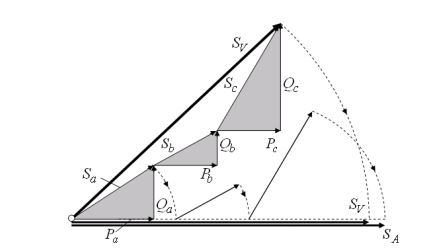
\includegraphics{2Marco/intergeo}
\caption{Potencias aparentes aritméticas y vectoriales} \cite{A30}
\label{fig:inter}
\end{figure} 

\subsubsection{Factor de potencia aritmético y del vector }

\begin{equation}\label{EQ54}
PF_{V}=\frac{P}{S_{V}}\\
\end{equation}
$PF_{A}=\frac{P}{S_{A}}$\\

Una línea trifásica que abastece a uno o más clientes debería ser vista como un solo camino, una entidad que transmite la energía eléctrica a lugares donde es convertida en otras forma de energía. Esta mal ver cada fase como una ruta de energía independiente.\cite{A30}\\

\subsubsection{Potencia aparente efectiva}

Este concepto asume un circuito balanceado virtual que tiene exactamente las mismas líneas de perdidas como el circuito des balanceado actual. Para un sistema de 4 líneas, el balance de la perdida de potencia es expresado en la siguiente ecuación:\cite{A30}\\

\begin{equation}\label{EQ55}
r(I^2_{a}+I^2_{b}+I^2_{c}+\rho I^2_{n})=3rI^2_{e}\\
\end{equation}
Donde:\\\\
$r$			es la resistencia\\
$I_{n}$		es la corriente actual (rms)\\
$r_{n}$		Es el cable neutro de la resistencia\\

De las ecuaciones anteriores, la corriente equivalente de un sistema de 4 líneas es el siguiente:\\

\begin{equation}\label{EQ56}
I_{e}=\sqrt{\frac{I^2_{a}+I^2_{b}+I^2_{c}+\rho I^2_{n}}{3}}=\sqrt{(I^+)^2+(I^-)^2+(1+3\rho)(I^0)^2}\\
\end{equation}

Y para un sistema de tres hilos donde $I^0=0$\\

\begin{equation}\label{EQ57}
I_{e}=\sqrt{\frac{I^2_{a}+I^2_{b}+I^2_{c}}{3}}=\sqrt{(I^+)^2+(I^-)^2}\\
\end{equation}

\subsubsection{Factor de potencia efectiva}

\begin{equation}\label{EQ58}
PF_{e}=\frac{P}{S_{e}}\\
\end{equation}

\section{Ejercicio Práctico}

\subsection{Análisis de datos obtenidos de tres cargas no lineales}

A continuación, se muestra el análisis de los datos obtenidos por el circutor de tres computadores de los ETM de la Universidad Santo Tomas en la sede central, siguiendo las normas establecidas para cada caso a nivel nacional. \\
El circutor no posee una memoria que almacene los datos medidos, por tal razón, los datos obtenidos se transmiten en tiempo real por comunicación serial a un computador por medio de un programa realizado en Visual Studio, donde se pueden adquirir las medidas de potencia, tensiones, voltajes, THDi, THDv, en una hoja de cálculo.\\
Las medidas tomadas y el análisis de estas, se realizaron tomando como referencia la norma NTC 1340 (tercera actualización) y el IEEE 1159, el cual establece el tiempo de muestreo para el monitoreo de calidad de energía eléctrica que es mayor a un minuto para sistemas de larga duración en variaciones de rms.

\begin{table}
\begin{center}
\begin{tabular}{ |c|c|c|c|c|c|c|c|c| } 
\hline
Nombre & Fecha & Hora & Prom & Min & Max & Muestras & Duración & Unidades\\
\hline
Frecuencia & 18/05/2018 & 18:13 & 60 & 60 & 60 & 30 & 6:00 & min:s\\
\hline
\end{tabular}
\end{center}
\caption{Datos de caracterización de frecuencia}
\label{tab:ejercicio-frecuencia}
\end{table}



\begin{figure}[H]
\centering
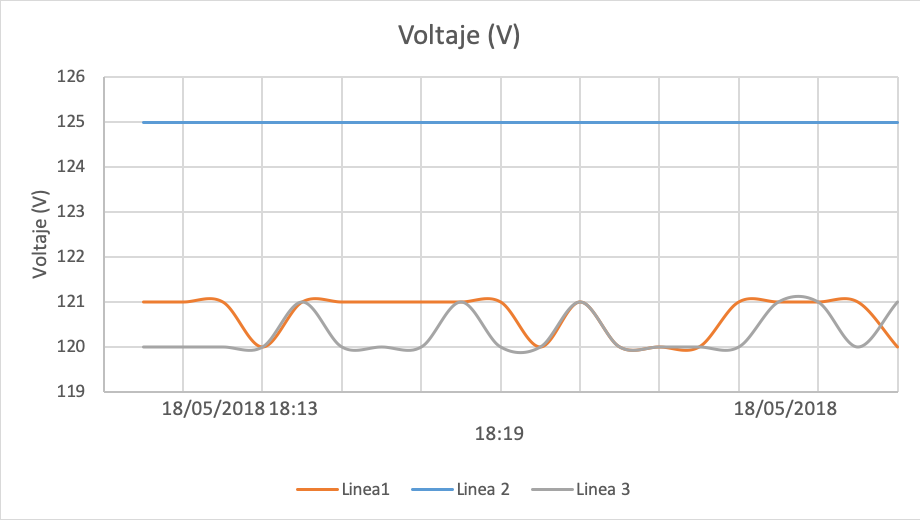
\includegraphics{2Marco/voltaje-rms}
\caption{Voltaje RMS (Autoria propia)} 
\label{fig:voltaje-rms}
\end{figure} 

Según la norma NTC 1340 (Tercera actualización) expresa que el 100\% de los valores medidos en el rango establecido del IEEE 1159, deben estar dentro del intervalo definido en la figura \ref{fig:tension-nominal}

\begin{figure}[H]
\centering
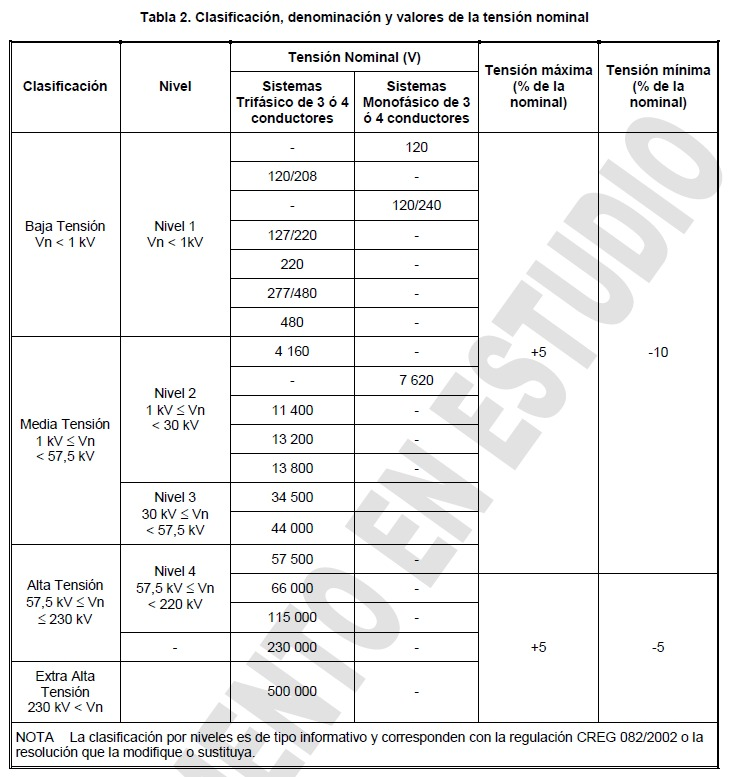
\includegraphics[width = 10cm]{2Marco/tension-nominal}
\caption{Clasificación, denominación y valores tensión nominal} \cite{A44}
\label{fig:tension-nominal}
\end{figure} 

Con los valores de la figura \ref{fig:voltaje-rms} se evidencia que los valores máximos y mínimos de VRMS, cumplen con los porcentajes establecidos.

\begin{align*}
X1 = \frac{Vmaxl1}{120} = \frac{121}{120} = 1.008;\;\mathbf{ 0,8\% VRMS} \\\\
X2 = \frac{Vmaxl2}{120} = \frac{125}{120} = 1.041;\;\mathbf{ 4.1\% VRMS} \\\\
X3 = \frac{Vmaxl3}{120} = \frac{121}{120} = 1.008;\;\mathbf{ 0,8\% VRMS}
\end{align*}
\textbf{Porcentaje máximos de volatjes}\\
\begin{align*}
&y1 = \frac{Vminl1}{120} = \frac{120}{120} = 1.00;\;\mathbf{ 0\% VRMS} \\\\
&y2 = \frac{Vminl2}{120} = \frac{125}{120} = 1.041;\;\mathbf{ 4.1\% VRMS} \\\\
&y3 = \frac{Vminl3}{120} = \frac{120}{120} = 1.00;\;\mathbf{ 0\% VRMS}
\end{align*}
\textbf{Porcentaje mínimos de volatjes}\\

\begin{table}
\begin{center}
\begin{tabular}{ |c|c|c| } 
\hline
VRMS & MÁXIMO & MÍNIMO\\
\hline
L1V & 0.8\% & 0\%\\
\hline
L2V & 4,1\% & 4,1\%\\
\hline
L3V & 0.8\% & 0\%\\
\hline
\end{tabular}
\end{center}
\caption{Tabla de rangos máximos y mínimos de VRMS}
\label{tab:rangos-vrms}
\end{table}

Al comparar los datos de la tabla en la figura \ref{fig:tension-nominal} con la tabla \ref{tab:rangos-vrms}, se afirma que la tensión nominal de las cargas cumple con los intervalos establecidos en la norma NTC 1340.\\

\begin{table}[!htbp]
\begin{center}
\begin{tabular}{ |c|c|c|c|c|c|c|c|c| } 
\hline
Nombre & Fecha & Hora & RMS & Min & Max & Unidades & Duración & Unidades\\
\hline
L1 Irms & 18/05/2018 & 18:13 & 605,1 & 537 & 808 & mA & 6:00 & min:s\\
\hline
L2 Irms & 18/05/2018 & 18:13 & 624,1 & 576 & 790 & mA & 6:00 & min:s\\
\hline
L3 Irms & 18/05/2018 & 18:13 & 576,5 & 553 & 730 & mA & 6:00 & min:s\\
\hline
\end{tabular}
\end{center}
\caption{Datos de caracterización de corriente}
\label{tab:ejercicio-corriente}
\end{table}

\begin{figure}[H]
\centering
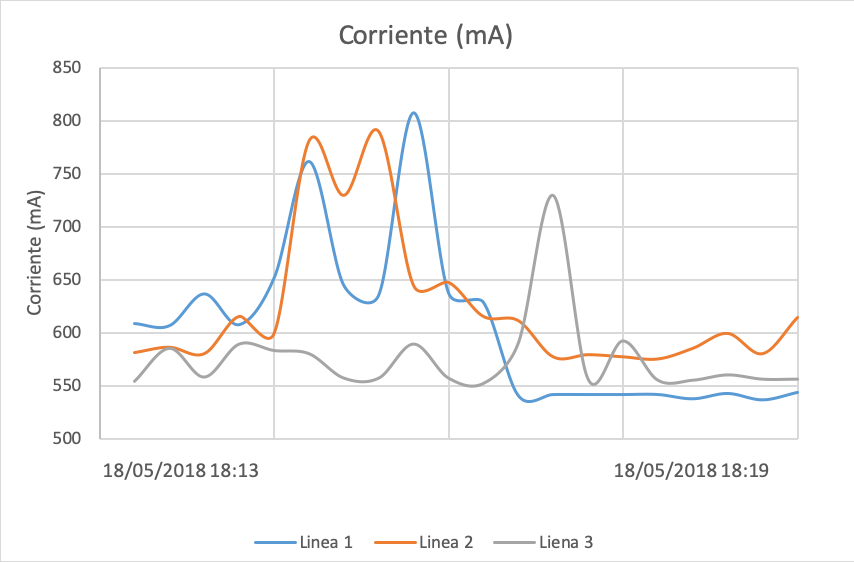
\includegraphics{2Marco/corriente-rms}
\caption{Corriente RMS (Autoria propia)} 
\label{fig:corriente-rms}
\end{figure} 

La figura \ref{fig:corriente-rms} corresponde a la corriente consumida dentro del intervalo ya establecido, se observa que los valores cambian en un rango de 300 mA, debido al uso que le aplican al computador.

\begin{table}[!htbp]
\begin{center}
\begin{tabular}{ |c|c|c|c|c|c|c|c|c| }
\hline
Nombre & Fecha & Hora & RMS & Min & Max & Unidades & Duración & Unidades\\
\hline
L1 THDv & 18/05/2018 & 18:13 & 2,9 & 2 & 3 & \% & 6:00 & min:s\\
\hline
L2 THDv & 18/05/2018 & 18:13 & 2,85 & 2 & 3 & \% & 6:00 & min:s\\
\hline
L3 THDv & 18/05/2018 & 18:13 & 2,9 & 2 & 3 & \% & 6:00 & min:s\\
\hline
L1 THDi & 18/05/2018 & 18:13 & 40,44 & 34,2 & 45,4 & \% & 6:00 & min:s\\
\hline
L2 THDi & 18/05/2018 & 18:13 & 39,75 & 25,6 & 44,9 & \% & 6:00 & min:s\\
\hline
L3 THDi & 18/05/2018 & 18:13 & 40,45 & 30,9 & 44,5 & \% & 6:00 & min:s\\
\hline
\end{tabular}
\end{center}
\caption{Distorsión armónica en corriente y voltaje}
\label{tab:distorsion-armonica}
\end{table}

\begin{figure}[H]
\centering
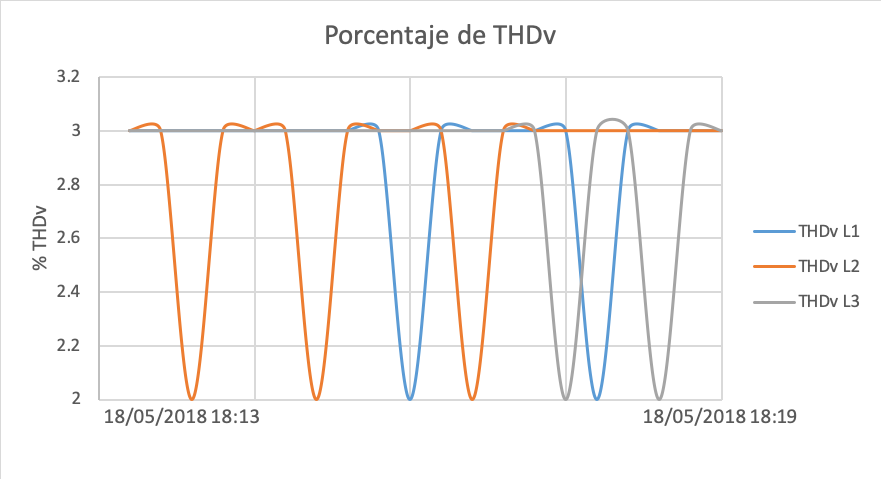
\includegraphics{2Marco/porcentaje-thdv}
\caption{Porcentaje de $THD_{V}$ (Autoria propia)} 
\label{fig:porcentaje-thdv}
\end{figure} 

\begin{figure}[H]
\centering
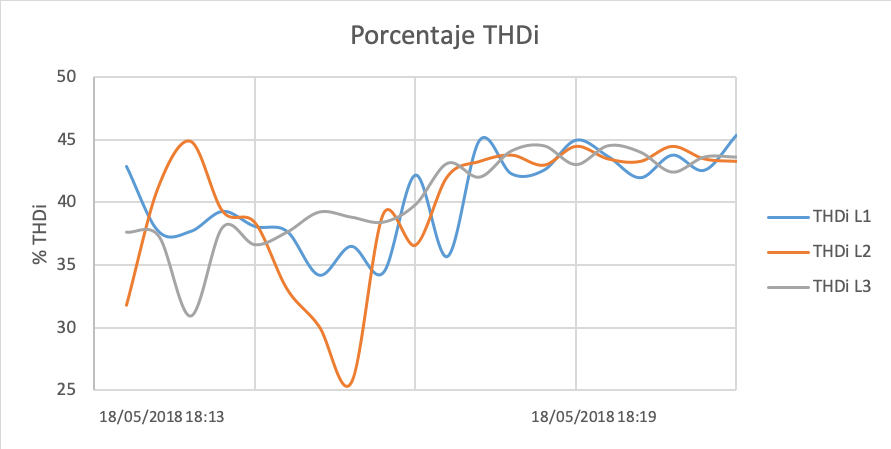
\includegraphics{2Marco/porcentaje-thdi}
\caption{Porcentaje de $THD_{I}$ (Autoria propia)} 
\label{fig:porcentaje-thdi}
\end{figure} 

Los datos de distorsión armónica reflejados en la tabla \ref{tab:distorsion-armonica} y las figuras \ref{fig:porcentaje-thdv}, \ref{fig:porcentaje-thdi} dan a entender como esta afectando las cargas no lineales en el sistema. Según el estándar IEEE 519 en el capitulo 11.1 indica el límite máximo que debe tener el THD en tensión (5\%), de acuerdo en la figura \ref{fig:porcentaje-thdv}, los THD de tensión no exceden el valor indicado anteriormente, por lo tanto, la red está cumpliendo la normatividad internacional.\\ 
En los THD de corriente, para su análisis es necesario hallar la distorsión de la demanda total con la siguiente ecuación:\\

\begin{equation}\label{EQ63}
TDD=\frac{I1*THD}{IL}\\
\end{equation}
\textbf{Ecuación \ref{EQ63}. Distorsión de demanta total.}

La corriente de carga (IL1) se toma el promedio de la tabla de datos que se obtiene por medio del CIRCUTOR de la siguiente manera:

\begin{align*}
&IL1 = L1Irms\;\;\; RMS = 605.1\\
&I_{1a1} = I_{L1} - (I_{L1} * 0.4044) = 0.605 - (0.605 * 0.4044) = 0.3603
\end{align*}

Aplicando la ecuación \ref{EQ63}

\begin{align*}
TDD_{1} = \frac{I_{1a1}*THD_{1}}{I_{L1}} = \frac{0.3603*0.4044}{0.605} = 0.2408 = 24.08\%
\end{align*}

La corriente de carga (IL2) se toma el promedio de la tabla de datos que se obtiene por medio del CIRCUTOR de la siguiente manera:

\begin{align*}
&IL2 = L2Irms RMS = 624.1\\
&I_{1a2} = I_{L2} - (I_{L2} * 0.3975) = 0.624 - (0.624 * 0.3975) = 0.3760
\end{align*}

Aplicando la ecuación \ref{EQ63}

\begin{align*}
TDD_{2} = \frac{I_{1a2}*THD_{2}}{I_{L2}} = \frac{0.3760*0.3975}{0.624} = 0.2395 = 23.95\%
\end{align*}

La corriente de carga (IL3) se toma el promedio de la tabla de datos que se obtiene por medio del CIRCUTOR de la siguiente manera:

\begin{align*}
&IL3 = L3Irms RMS = 576.5\\
&I_{1a3} = I_{L3} - (I_{L3} * 0.4045) = 0576 - (0.576 * 0.4045) = 0.2330
\end{align*}

Aplicando la ecuación \ref{EQ63}

\begin{align*}
TDD_{3} = \frac{I_{1a3}*THD_{3}}{I_{L3}} = \frac{0.2330*0.4045}{0.576} = 0.1636 = 16.36\%
\end{align*}\\

\begin{table}[!htbp]
\begin{center}
\begin{tabular}{ |c|c| } 
\hline
Corrientes & TDD\\
\hline
AL1 & 24.08\%\\
\hline
AL2 & 23.95\%\\
\hline
AL3 & 16.63\%\\
\hline
\end{tabular}
\end{center}
\caption{TDD de corrientes}
\label{tab:tdd-corriente}
\end{table}

Tomando como referencia la figura \ref{fig:límites-corriente}, la cual está en el estándar IEEE 519 y la tabla \ref{tab:tdd-corriente}, se observa que los resultados de TDD obtenidos en las ecuaciones anteriores están dentro del rango aceptado en el estándar, comprobando que el sistema está trabajando en un estado estable. 

\begin{figure}[H]
\centering
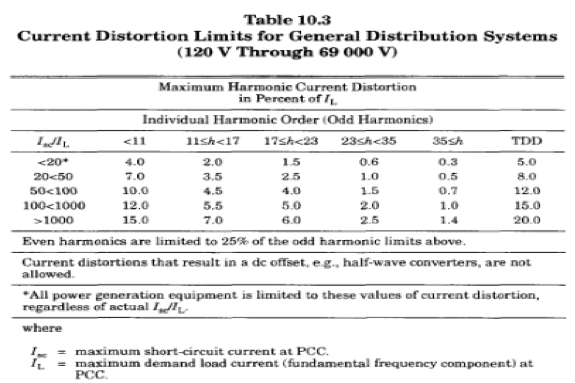
\includegraphics{2Marco/limites-distorsion-corriente}
\caption{Límites de distorsión de corriente para sistemas de distribución general} \cite{A45}
\label{fig:límites-corriente}
\end{figure} 

\section{Desarrollo de Software}

El desarrollo de software es un campo de la ciencia computacional dedicado a la creación, diseño, implementación y soporte de software.

El software se compone de una serie de instrucciones o programas que le dicen al computador que debe hacer. Es independiente del hardware y hace a los computadores programables.  \cite{A31}

\subsection{Programación Orientada a Objetos}

La programación orientada a objetos (POO) es un paradigma de programación  basado en convertir objetos que puedan ser tangibles o intangibles a objetos digitales los cuáles tienen métodos y propiedades. Esto genera ventajas en modularidad y reusabilidad en código. Los objetos que usualmente son instancias de clases, son utilizados para interactuar uno con otro para diseñar aplicaciones y programas de computadores. \cite{A32}

\subsection{Desarrollo Web}

El desarrollo web es una área del desarrollo de software la cuál construye, crea y mantiene sitios web. Dentro de su funcionamiento incluye el diseño web, publicación web y administración de base de datos. \cite{A33}

\subsection{Frontend}

Frontend se entiende como la parte de un programa en la cuál se crea una interfaz de usuario para que el programa interactue con las personas. Los lenguajes principales desarrollo del frontend son Html5, Javascript y Css 3; aunque hay muchos frameworks facilitan la creación de frontend, cómo lo son: React, Angular2+, Vuejs y Bootsrap entre otros.

\subsection{Backend}

En la capa de arquitectura de un proyecto de software, el backend no es accesible por los usuarios ya que este es el encargado de ejecutar todas las funciones y la lógica del sistema, administra, guarda y envía información a la base de datos.

\subsection{REST}

REST se compone de una serie de principios de comunicación web en la cual se diseñan servicios web orientados a recursos de sistemas, incluyendo como los estados de los recursos son ubicados y transferidos a través del protocolo HTTP por un gran rango de clientes que usan distintos lenguajes de programación.  \cite{A37}


\section{Fourier}
\subsection{Transformada de Fourier}
La transformada de Fourier transforma una señal que depende del tiempo en una señal que depende de la frecuencia (tiempo continuo a tiempo discreto).
\begin{equation}
F(g(t))=G(f)=\int_{-\infty}^{\infty}g(t)e^{-i2\pi ft}dt   
\end{equation}
Se define como la transformada de Fourier. \cite{A34}
\begin{equation}
F^{-1}(G(f))=g(t)=\int_{-\infty}^{\infty}G(f)e^{i2\pi ft}df   
\end{equation} 
Se define como  la inversa de Fourier. \cite{A34}

\subsection{Teorema de muestreo de Nyquist-Shannon}
Sea una señal de \textit{x(t)} de  finita y de banda  limitada  a B, entonces:
\\

$x(t)=\dfrac{1}{\pi}\sum_{n=-\infty}^{\infty} x(\dfrac{n}{2B})\dfrac{\sin(\pi(2Bt-n)) }{2Bt-n}$
\cite{A35}\\

para reconstruir una señal limitada entre la banda B es necesario tener una señal de muestreo de 2B, esta frecuencia se denomina frecuencia de Nyquist.

\begin{equation}
F_{min}>2f
\end{equation}
Donde:\\
F$_{min}$ = Frecuencia mínima de muestreo.\\
f = Frecuencia fundamental de la señal.

\subsection{Transformada rápida de Fourier (FFT) }
Todas las señales periódicas pueden ser representadas en sumatorias de Fourier, de esta sumatoria de Fourier se puede sacar la transformada de Fourier discreta calculando un tiempo finito, esta transformada se define como:
\begin{equation}
X[k]=\sum_{n=0}^{N-1}x[n]W_{N}^{kn} ; \\   k = 0,1,2,3...N-1
\end{equation}
donde $W_{N}=e^{-j\dfrac{2\pi}{N}}$\\
La FFT surge en dividir el tiempo, es decir en la descomposición en transformadas de Fourier Discretas mas simples, para esto se asume que la N es potencia de 2, descomponiendo la como: 

\begin{equation}
X[k]=\sum_{r=0}^{N/2-1}x[2r](W_{N/2})^rk + W_{N}^K \sum_{r=0}^{N/2-1}x[2r+1](W_{N/2})^rk
\end{equation}

donde $W_{N/2}=e^{-j\dfrac{2\pi}{N/2}}$, N siendo el número de muestras. \cite{A36}\\

Esta manera es la que usan la mayoría de conversares análogos digitales y procesadores. 


\section{Convertidores ADC}
El convertidor análogo digital (ADC) fue creado para representar en una palabra digital el nivel de voltaje existente en una en una entrada análoga, transformándola en una señal binaria de un número de muestras (N), en la electrónica la resolución de la señal de entrada la da la cantidad de bits disponibles para la conversión, entre mas grande sea la cantidad de bits, mayor es la resolución de la señal y mas confiable es ésta. 

\section{Internet de las cosas}

El concepto de internet de las cosas o por su sigla en ingles (IoT) - internet of things, tiene como objetivo conectar lo desconectado, esto significa que algún dispositivo que no tenga comunicación con la red lo pueda tener y así puedan interactuar con las personas y otros objetos. IoT es una tecnología de transición en donde los dispositivos permitiran sensar y controlar el mundo fisico haciendo los objetos inteligentes y conectandolos a través de una red inteligente. Esta transición de volver un dispositivo intelegente se puede realizar de distintas formas pero la más común para empezar es la Raspberry. \cite{A38}

\subsection{Raspberry pi 4}

Las Raspberry Pi 4 es la nueva generación de computadores soportando más memoria RAM y un mejor rendimiento en CPU, GPU y puertos de entrada y salida. Esta tarjeta cuenta con conectividad Bluetooth 2.0, USB, Red y Wifi, también tiene el protocolo de comunicación I2C el cual permite comunicarse con sistemas digitales electrónicos con el fin de recibir y transmitir información y por medio de la conectividad Wifi, se puede hacer conectividad a la red dispositivos que no tienen conectividad. El mayor beneficio de esta funcionalidad de la Raspberry hace posible el concepto de IoT y así puede haber una interacción entre las personas y los dispositivos. \cite{A39}